\documentclass[dissertation.tex]{subfiles}
\begin{document}

\chapter[Identifying Optimal Biomarkers for Clinical Tests][Finding Optimal Biomarkers]{Identifying Optimal Biomarkers for Clinical Tests}
\label{chap:messina}


\emph{Thesis: Binary decision stump classifiers can be efficiently trained on high-throughput biomarker data, and provide a principled way to translate large multi-measurement research data into simple but high-performance clinical tests.}


\paragraph{Summary}


\section{Introduction}

Research and molecular pathology laboratories take strikingly different approaches to the measurement of biomarkers in patient samples.  Research work favours costly manual techniques, which quantify a large number of biomarkers in a relatively small number of samples.  Conversely, pathology laboratories make extensive use of highly automated turnkey systems, to robustly measure a relatively small number of biomarkers in a large number of samples.  In keeping with this divide, research and pathology laboratories often use very different technologies for the measurement of the same type of biomarker, such as RNA sequencing in research, and quantitative PCR in the clinical realm.  This difference in base technology, and the generally increased variability of clinical samples over research ones~\cite{Hewitt2008}, complicates the translation of discoveries in research into application in the clinic.

Although difficult, this translation of research discoveries into clinical practice is absolutely necessary.  Research and pathology techniques are complementary: biomarker discovery requires research techniques capable of interrogating a huge number of potential biomarkers, but the \emph{application} of any discoveries must use pathology techniques that can reliably and economically handle a potentially huge number of patient samples.  Finding effective ways to translate research findings into clinical application is critically important.  This problem can be approached from two angles: by harmonising measurement technology between research and diagnostic laboratories, or by identifying lead biomarkers in the research laboratory that have a high likelihood of effectively translating to diagnostic measurement.  The former approach may represent a long-term solution, but does not reflect the current state of technology.  To implement the latter approach requires bioinformatic techniques that can search large bodies of research measurement data, to identify a small number of biomarkers that are most likely to make good diagnostic tests.

Effective clinical tests must satisfy a number of requirements, which can be used to guide the translation of a research finding into a clinical tool.  Ideally, a clinical diagnostic or prognostic test should be based on the measurement of only a small number of biomarkers~\cite{Lesko2001, Pepe2001}.  Additionally, it should be highly robust to technical effects, and the inevitable variation in sample quality and handling that comes with clinical specimens~\cite{Hewitt2008}.  The results of most tests will be interpreted as a simple binary variable\footnote{For example, disease versus not diseased, responder versus non-responder, or poor prognosis versus good prognosis.}, and the detection performance of this binary variable should match the particular clinical application~\cite{Pepe2001}.  Taking all these requirements into account, a technique to translate discovery biomarker measurements into a clinical test should be able to process measurements of thousands of biomarkers to identify those single biomarkers that, when their level is thresholded, yield a particular class separation performance, with maximal robustness to technical effects.

Existing methods for the mining of research data for potential biomarkers do not meet these requirements.  For both diagnostic and prognostic endpoints, common biomarker prioritization techniques either do not provide fine control of classification accuracy and robustness, or yield sets of biomarkers that are far too large to practically deploy.  Two broad strategies are generally employed to identify biomarkers in large research data sets: univariate statistics, and machine learning.  The first strategy encompasses approaches such as per-biomarker regression tests for association between the biomarker and a sample group or outcome, and the second covers the use of algorithms such as \glspl{SVM} to construct high-performance predictors of group or prognosis from the measurements of many biomarkers.

Univariate statistic approaches identify single biomarkers of interest, but supply no guarantee as to the suitability of these biomarkers for translation into clinical tests.  These statistics are designed to identify differences in average value between two groups, not to construct classifiers.  Significance testing and classifier learning are distinct problems, and usually have different solutions: a biomarker that shows a statistically significant difference in signal between two groups may still be a poor classifier; and vice versa (\fref{fig:messina-example-stats-class}).  Univariate tests also do not take the particular requirements of a clinical problem into account.  For example, consider two tests for the same disease -- one test is intended to be used as a population screen, and the other to rule out a suspected diagnosis.  These two tests would have very different performance requirements, and quite possibly would be best served by two different biomarkers.  Univariate test approaches to candidate biomarker selection cannot take this nuance into account, which further limits their usefulness for biomarker selection.
% These special test performance requirements can be accommodated by machine learning algorithms, but the classifiers produced by these algorithms are also usually poorly-suited to clinical test development.
% Mention that this is because of the sqrt(n) factor in the tests?  Testing hypotheses on population mean, not on population distrib.

\begin{figure}[!htbp]
  \centering
  \vspace{1cm}
  \subbottom[Poor classification]{
    \def\svgwidth{.4\linewidth}
	\input{messina_class_test_comparison_a.pdf_tex}
    \label{fig:messina-example-stats-class-stat}}
  \hspace{1cm}
  \subbottom[Good classification]{
    \def\svgwidth{.4\linewidth}
	\input{messina_class_test_comparison_b.pdf_tex}
    \label{fig:messina-example-stats-class-class}}
  \caption[Statistical significance does not imply good classification ability]{Statistical significance does not imply good classification ability.  The left and right panels show the distributions of two hypothetical biomarkers, $a$ and $b$, in two sample classes, shown in orange and green.  The intent is to construct a single-feature classifier separating the two sample classes.  The levels of biomarker $a$ (left panel) are significantly different between the two classes, but the large overlap in distributions would make it a poor choice for a classifier, with sensitivity and specificity both approximately $0.6$.  Conversely, biomarker $b$ (right panel) could be used to form an effective threshold-based classifier, with sensitivity and specificity each around $0.8$.  This comparison also demonstrates the unsuitability of many univariate statistical tests for classifier selection: for example, biomarker b does not show significantly different expression between the groups by the t and Mann-Whitney U tests, although it does by the more general Kolmogorov-Smirnov test (data not shown).}
\label{fig:messina-example-stats-class}
\end{figure}

Machine learning algorithms can produce highly accurate classifiers matching given performance requirements~\cite{Bach2006}, but these classifiers generally rely on combining information from a large number of biomarkers.  This has not entirely prevented multi-gene tests based on these classifiers from achieving clinical use (an early example of a multi-gene clinical test is MammaPrint\texttrademark, a simple linear classifier based on measurements of 70 transcripts~\cite{Veer2002}), but does drastically increase the complexity of translation from the research laboratory to the clinical, and the final cost of the test (for MammaPrint, approximately \fcardinal{4200} USD per patient).  As well as being difficult to translate into a clinical diagnostic, high-performance multi-feature classifiers require care when training~\cite{Aliferis2009}, their complex workings usually defy human interpretation~\cite{Breiman2001b}, and their complexity often simply isn't required for good classification~\cite{Grate2005}.  Many approaches are available to limit the number of biomarkers in classifiers returned by machine learning algorithms~\cite{Guyon2003}, but as the number of biomarkers is reduced to one, this generally comes at the cost of performance (TODO cite?).  For the limiting case of single-biomarker classifiers and prognostics, a machine learning algorithm designed exclusively for the task is needed.

To address this need, in 2009 I reported the Messina algorithm, for the efficient cost-sensitive training of single-feature binary decision stump classifiers~\cite{Pinese2009}.  The classifiers found by Messina use the abundance of a single biomarker to place samples into two groups: one containing samples with biomarker levels below a threshold, and the other containing samples with biomarker levels at or above the threshold.  Given measurements of many biomarkers in a set of samples from two groups, Messina identifies the biomarkers, and their optimal thresholds, that will separate the two groups well.  Messina could be used to address two problems: the selection of biomarkers that are well-suited for development into single-measurement diagnostic tests, and the identification of biomarkers with differential signal between two sample groups.  The latter functionality was the focus of the original Messina paper, which demonstrated that Messina was a strong alternative to more classical tests of differential expression, that allowed the user to smoothly trade robustness to outliers against sensitivity to subtle changes in expression.  Messina was recommended by an independent comparison of outlier differential expression methods~\cite{Karrila2011}, but remains a relatively limited tool: Messina is only available as a standalone program, and its objective function is hard-coded for binary classification, and so it can not generate more general classifiers, such as for prognosis.

Tools to identify biomarkers that can yield accurate estimates of prognosis remain relatively crude, compared to those for classification problems.  As discussed in \Cref{chap:nomogram}, there is a pressing need in \gls{PDAC} for effective methods to preoperatively stage patients.  Biomarkers of prognosis can be measured preoperatively, but the S100A2 and S100A4 markers tested in \Cref{chap:nomogram} were relatively poor at predicting outcome following resection of \gls{PDAC}.  S100A2 and S100A4 were identified following only a small candidate screen, and it is reasonable to expect that a global search for \gls{PDAC} biomarkers of prognosis will yield candidates with better performance.  Prognostic tests have the same clinical translation requirements as diagnostic tests: they must be based on a small number of biomarker measurements, and by simple thresholding of these measurements, yield a robust prediction of differential outcome.  Machine learning algorithms such as random forests and \glspl{SVM} have been adapted to the prediction of outcome, but suffer the same general problem of machine learning solutions: too many biomarkers must be measured to achieve accurate prediction.  Most univariate statistics approaches also suffer the same problem as their classification counterparts, by failing to take the particular class separation needs of the application into account.  These problems with conventional approaches have led to the common use of ad-hoc analyses when identifying biomarkers of prognosis.

The poor suitability of conventional approaches for identifying biomarkers of prognosis has led to the common use of ad-hoc analyses for this problem, but these usually perform very poorly.  Methods in common use are the median cut, in which the cohort is divided into two groups by the median value of each biomarker, and then a log-rank test performed on these two groups; and the so-called `optimal' cut, in which many cutpoints are tried, and the best log-rank statistic is used as the final test statistic.  The median cut approach presupposes that the poor- and good-prognosis subgroups in the data are equal in size, and has poor power if this is not the case, and the `optimal' cut procedure is decidedly non-optimal, with an unsurprising high false detection rate due to uncorrected multiple testing.  Although discussion of the significant deficiencies in these approaches has been in the medical literature for over twenty years~\cite{Altman1994}, they continue to see routine use and further development~\cite{Budczies2012,Camp2004,Chorlton2014,Yau2010}.  A natural approach to correcting the `optimal' procedure is by incorporating multiple testing correction, and software is available to perform this as \texttt{R} package \texttt{maxstat}~\cite{Chorlton2014,Hothorn2003}.  However, in common with more conventional univariate approaches, \texttt{maxstat} and similar methods do not allow for control over any desired aspects of the prognostic classifier, such as the hazard ratio between the poor- and good-prognosis groups, or the relative group sizes.  As in the classification case, a biomarker selection procedure specifically designed for clinical translation is needed.

In this chapter I present Messina2, a general algorithm for single-feature decision stump classifier learning.  Like its predecessor Messina, Messina2 aims to produce maximally robust classifiers that satisfy user-supplied performance requirements.  Unlike Messina, Messina2 accepts any performance metric, and so can be used to create binary classifiers for any task, including diagnosis and prognosis.  Messina2's emphasis on maximally robust classifiers means that the biomarkers that it selects are especially well suited for translation to the clinical diagnostic laboratory, helping to address the divide between research discovery and clinical application.  To facilitate Messina2's use in bioinformatic workflows, it has been made into the \texttt{R} package \texttt{messina}, available as part of the Bioconductor project~\cite{Gentleman2004}\footnote{The version of Messina2 used for this thesis is not yet in the latest Bioconductor release.  To access the thesis version, clone the \texttt{thesis} branch from the Bitbucket repository \texttt{marpin/r-messina}, or from \texttt{R}, with \texttt{devtools} installed, run the command \texttt{ devtools::install\_bitbucket("marpin/r-messina", ref = "thesis")}.}.  This chapter will describe the general framework of binary decision stump classifiers, detail the Messina2 algorithm and how it differs from Messina, and demonstrate its characteristics and performance relative to other techniques.  An application to the problem of identifying better prognostic biomarkers in pancreas cancer will illustrate the utility of Messina2 in real data.

\section{Messina2}
Messina and Messina2 are algorithms that take as input measurements of biomarker abundance in a number of samples, and return as output decision stump classifiers that can separate the input samples into two groups.  For Messina, these groups are based on user-supplied sample labels, such as cancer and non-cancer, and the classifiers are designed to separate these two sample types as robustly as possible, whilst still meeting user-supplied minimum sensitivity and specificity requirements\footnote{Here sensitivity and specificity are used in their binary classification sense.  In a binary classification problem (for example, a diagnostic test to detect the presence of a disease, where the result is either `diseased,' or `not diseased,' with no intermediate `uncertain'), a given classifier tested on a population of samples will have associated rates of true positive, true negative, false positive, and false negative calls.  The sensitivity of this classifier on that population is then the true positive call rate divided by the total positive sample rate, and the specificity is the true negative call rate divided by the total negative sample rate.  Symbolically, let $R_{ab}$ be the rate at which a sample which is truly of class $a$ is called as class $b$, $a, b \in \{0,1\}$, where $1$ represents the positive class, and $0$ the negative.  Then, $\mathrm{Sens} = p_n = R_{11} \div R_{1\bullet}$, and $\mathrm{Spec} = p_c = R_{00} \div R_{0\bullet}$.}.  Messina2 is more general, producing classifiers that satisfy a user-supplied objective function as robustly as possible.  One specific form for this objective function yields results very similar to those of Messina, but through use of different objective functions, Messina2 can be used to address effectively any binary separation problem, such as the creation of decision stump classifiers to distinguish between good- and poor-prognosis patients.  This chapter will primarily describe Messina2, drawing comparisons to Messina where appropriate.

\subsection{Messina2 framework}
\paragraph{Decision stump classifiers}
A decision stump classifier is a very simple classifier that is equivalent to a one-level decision tree~\cite{Iba1992}.  In the binary variant employed by Messina2, an unknown sample is assigned to one of two classes, depending on whether that sample's abundance of a certain biomarker is above, or below, a threshold value.  More precisely, let the abundance of a certain biomarker in sample $i$ be $x_i$.  Suppose sample $i$ can be one of two classes, here called 0 and 1, and the goal is to predict the class of $i$ based on $x_i$.  Then, a decision stump classifier will predict the class of $i$, $w_i$, as $w_i = [ x_i d \geq t d ]$, where $t$ is the threshold level at which the predicted class changes, and $d \in {-1, 1}$ is the classifier direction: if $d = 1$, then values of $x$ at or above $t$ are predicted to be class 1, if $d = -1$, then values of $x$ of at least $t$ are predicted to be class 0.  This situation, for $d = 1$, is shown in the top two lines of \fref{fig:mess-thresh-1}.  A decision stump classifier for a given biomarker is completely specified by the values of $t$ and $d$; finding values for these two variables that in some way meet desired criteria is the goal of classifier training.

\begin{figure}[!htbp]
\centering
\def\svgwidth{\linewidth} 
\input{messina_threshold_1.pdf_tex}
\caption[]{TODO}\label{fig:mess-thresh-1}
\end{figure}

\paragraph{Objective function}
To identify optimal values of $t$ and $d$ for a given problem, Messina2 employs the concept of an \emph{objective function}.  Suppose that we have measurements of a certain biomarker $x$ for each of $n$ samples.  For each sample, we also have the value of a dependent variable $y$; this may be a biological class (eg. cancer or non-cancer), a survival time, or any multidimensional measurement.  Our goal is to create a decision stump classifier that operates on $x$, so that the two groups of samples so created are somehow `well-separated' in their values for $y$.  The concept of `well-separated' is left deliberately vague, because it is under the control of the user, via the objective function.  Common examples of good separation would be: for cancer diagnosis, most of the cancer samples are in one group, and most of the non-cancer samples are in the other; and for survival, there is a large difference in prognosis between the two sample groups.  We formalise this concept of objective function as follows.  Let the objective function $f: (\mathbb{B}^n, \mathbb{Y}^n) \rightarrow \mathbb{B}$ accept an $n$-tuple of sample groupings (as defined by $t$ and $d$) $w$, and an $n$-tuple of dependent values $y$, and return a binary value -- $\mathrm{true}$ if the split of $y$ given by $w$ is desirable, otherwise $\mathrm{false}$.  The operation of the objective $f$ for a binary $y$ is illustrated in \fref{fig:mess-thresh-1}.  Here $w$ is expressed as a function of $t$ and $d$, and the particular split given is considered desirable, so that $f(w(t, d), y) = \mathrm{true}$.  For a given $x$, $y$, and $f$, it is possible that many values of $t$ and $d$ satisfy the objective function, that is, $f(w(t, d), y) = \mathrm{true}$ does not have a unique solution in $(t, d)$.  In this case, a principled way to select a $(t, d)$ that is in some sense optimal, is required.

\paragraph{Margin}
A concept in machine learning is that of the \emph{margin}.  Informally, the margin describes the distance between the decision boundary (here, the threshold $t$) and the data, and is a measure of the confidence and robustness of a classifier: a classifier with a high relative margin has all observed data points safely `far away' from the decision boundary, and unlikely to change class following a perturbation.  Messina and Messina2 use a slightly different concept of margin, as the smallest distance that the decision boundary must move for the objective function to be violated.  Using the heuristic that classifiers with the greatest margin are the most robust, Messina2 chooses the optimal threshold $t^*$ as the midpoint of the largest real interval for which $f(w, y) = \mathrm{true}$, and selects the optimal direction $d^*$ as the one associated with $t^*$.  The intuition behind this selection is that such a choice of threshold and direction maximises the size of the smallest threshold perturbation that is necessary to make the classifier violate its performance requirements, that is, 
\begin{equation}
(t^*, d^*) = \argmax_{t,d} \mathrm{min}\left\{ \vert\delta\vert~:~\delta \in \mathbb{R} \wedge \neg f\left(~\left(~\left[x_i d \geq \left(t + \delta\right)d\right]~\right)_{i=1}^n, y\right) \right\}
\end{equation}
where $f([~[x_i d \geq (t + \delta)d]~]_{i=1}^n, y)$ is the value of the objective $f$ when the threshold $t + \delta$ is applied to the data $x$, with $\delta$ the perturbation.  This concept is illustrated in \fref{fig:mess-thresh-2}, which shows a wide region of potential thresholds $t$ in which the objective function $f$ is true.  The optimal threshold $t^*$ is in the centre of the largest interval for which $f$ is true, thereby maximising the margin $\Delta$.

\begin{figure}[!htbp]
\centering
\def\svgwidth{\linewidth} 
\input{messina_threshold_2.pdf_tex}
\caption[]{TODO}\label{fig:mess-thresh-2}
\end{figure}

\paragraph{Internal validation}
Messina2 considers all possible thresholds and directions $t \in \mathbb{R}, d \in \{-1,1\}$ when searching for $(t^*, d^*)$, and as such is at risk of overfitting the data, and reporting spurious classifiers.  To overcome this problem, Messina2 by default employs an outer bootstrap loop to verify that a classifier under consideration still satisfies the objective function $f$, when tested on holdout data.  Multiple bootstrap draws of the training data $(x, y)$ are made, and for each draw a Messina2 classifier is trained on the drawn samples, the trained classifier is used to separate the undrawn (so-called `out-of-bag') samples into two classes, and the objective $f$ is evaluated on the resulting two classes in the out-of-bag data.  Messina2 only returns classifiers for which the objective $f$ is $\mathrm{true}$ in at least half of the out-of-bag evaluations.  This outer bootstrap layer adds an additional level of stringency to the Messina2 results, but dramatically increases the runtime of the algorithm, and in some applications may not be required: the Vapnik–Chervonenkis dimension of a single-feature threshold classifier is $2$, and so Messina2's potential for overfitting is relatively low~\cite{Vapnik1999}, even before bootstrapping is performed.

\subsection{Objective functions}
Messina2 is designed to accept any objective function $f$, to allow custom analyses, but is also supplied with two reasonable default objective functions, designed to handle common tasks in classification and survival analysis.

\paragraph{Classification}
The objective function $f_M$ is designed to mimic the behaviour of the original Messina algorithm for classification and differential expression detection.  This function returns $\mathrm{true}$ if the data split $w$ separates the classes in $y$, with sensitivity and specificity at least as good as user-supplied minimum values:
\begin{align*}
f_M(w, y) &= \left[ p_n \geq l_n \wedge p_c \geq l_c \right] \\
p_n &= \frac{\sum_i{\left[ w_i \wedge y_i \right]}}{\sum_i{\left[ y_i \right]}} \\
p_c &= \frac{\sum_i{\left[ \neg w_i \wedge \neg y_i \right]}}{\sum_i{\left[ \neg y_i \right]}} \\
\end{align*}
In the above, $p_n$ and $p_c$ are the observed sensitivity and specificity, respectively, and $l_n$ and $l_c$ are their user-supplied minimum acceptable values.  When used with this objective function, Messina2 will return maximum-margin classifiers that separate the two groups defined in $y$ with at least the required minimum sensitivity and specificity.  When identifying lead biomarkers for the construction of a clinical test, the analyst can set the sensitivity and specificity requirements to values matching the intended application of the test, and be confident that the biomarkers reported by Messina2 will robustly separate the sample groups with at least this desired level of performance.  As sensitivity and specificity are closely related to a variable's \gls{CDF}, the objective function $f_M$ has close links with the data population \glspl{CDF}.  The optimal threshold $t*$ is the midpoint between values of $t$ for which the minimum sensitivity and specificity requirements are violated, and if the true \gls{CDF} were known for positive and negative sample populations, could be directly calculated from the inverse \glspl{CDF} (\fref{fig:mess-class-cdf-link}).

\begin{figure}[!htbp]
\centering
\def\svgwidth{\linewidth} 
\input{messina_class_cdfs.pdf_tex}
\caption[]{}\label{fig:mess-class-cdf-link}
\end{figure}

\paragraph{Prognosis}
The objective function $f_H$ is intended for survival analysis, where the goal is to identify biomarkers that can robustly separate a cohort into good- and poor-outcome groups.  Messina2 in this mode provides a more principled approach to thresholding biomarker levels for prognosis than median-cut or multiple-cut procedures.  $f_H(w, y)$ returns $\mathrm{true}$ if the approximate hazard ratio (using survival data in $y$) between the groups defined by $w$ is at least a user-supplied value.  The approximate hazard ratio is calculated from the log-rank test statistic, as:
\begin{align*}
f_H(s, y) &= \left[ \vert \log{p_h} \vert \geq \log{l_h} \right] \\
\log{p_h} &= Z\sqrt{\frac{4}{n_e}}
\end{align*}
where $p_h$ is the approximate hazard ratio achieved by the data split in $w$, $l_h$ is the minimum hazard ratio desired, $Z$ is the value of the log-rank test statistic\footnote{$Z$ is the signed log-rank test statistic, not to be confused with the $\chi^2$ statistic, which is also encountered.  $\chi^2 = Z^2$.}, and $n_e$ is the number of events in $y$.

\subsection{Algorithm}
Messina2 operates on each biomarker in a data set separately, reporting whether that biomarker can be used to build a threshold classifier with the desired performance characteristics, and, if so, the optimal such classifier.  The main entry point for Messina2 is given in as algorithm Messina2Entry (Algorithm \ref{alg:mess-messina2}), which performs bootstrap validation and final training for a single biomarker.  Messina2Entry calls algorithm MessinaCore (Algorithm \ref{alg:mess-core}), which performs the actual classifier training.  Although the preceding text described the search for the optimal $t$ as being over $\mathbb{R}$, this is not required in practice.  For given $d$, $w(t,d)$ only changes at values observed in $x$, so it is only necessary to check one value of $t$ per interval between consecutive values of $x$.  Candidate cutpoints satisfying this requirement are generated by the algorithm MakeCutpoints (Algorithm \ref{alg:mess-cutpoints}).  The resultant sparse $w(t,d)$ requires some care to recover correct threshold and margin values; the logic for this is in algorithm BestInterval (Algorithm \ref{alg:mess-bestinterval}), the operation of which is illustrated in \fref{fig:mess-bestinterval}.

\begin{algorithm}
  \KwData{Covariate measurements $x \in \mathbb{R}^n$, associated dependent values $y \in \mathbb{Y}^n$, objective function $f: (\mathbb{B}^n, \mathbb{Y}^n) \rightarrow \mathbb{B}$, minimum subclass fraction $b \in [0, \frac{1}{2})$, and a number of bootstrap rounds $r$.  $x$ is to be sorted in ascending order.  $\mathbb{Y}$ varies between modes of Messina2.}
  \KwResult{A 3-tuple.  If the fit failed, $(0, 0, 0)$.  Otherwise, optimal classifier parameters $(t^*, d^*, \Delta^*)$, with threshold $t^* \in \mathbb{R}$, direction $d^* \in \{-1, 1\}$, and margin $\Delta^* \in \mathbb{R}^+$.}

  \Begin {
  	$n_{\mathrm{pass}} \longleftarrow 0$\;
  	\For{$i \leftarrow 1$ \KwTo $r$}{
  		\tcp{Generate a bootstrap sample of (x, y)}
  		$(x_{\mathrm{in}}, y_{\mathrm{in}}, x_{\mathrm{out}}, y_{\mathrm{out}}) \longleftarrow \mathrm{BootstrapSample}\left( x, y \right)$\;
  		
  		\tcp{Train MessinaCore on this bootstrap sample}
  		$(t_{\mathrm{in}}, d_{\mathrm{in}}, \Delta_{\mathrm{in}}) \longleftarrow \mathrm{MessinaCore}\left( x_{\mathrm{in}}, y_{\mathrm{in}}, b, f \right)$\;
  		
  		\tcp{Assess performance of the MessinaCore classifier on the out-of-bag samples}
  		\If{$d_{\mathrm{in}} \neq 0$}{
  			$w_\mathrm{out} \longleftarrow \left(~\left[ x_{\mathrm{out}_j} d_{\mathrm{in}} \geq t_{\mathrm{in}} d_{\mathrm{in}}\right]~\right)_{j=1}^{\vert x_\mathrm{out} \vert}$\;
  			\If {$f\left(w_\mathrm{out}, y_{\mathrm{out}}\right) = \mathrm{true}$}{
  				$n_{\mathrm{pass}} \longleftarrow n_{\mathrm{pass}} + 1$\;
  			}
  		}
  	}
  	
  	\tcp{Did the in-bag trained classifiers satisfy out-of-bag performance requirements in at least half of the bootstrap rounds?}
  	\eIf{$r = 0 \vee n_{\mathrm{pass}} \geq \frac{1}{2}r$}{
	  	\tcp{Yes; return the fit on the full data}
  		\KwRet{$\mathrm{MessinaCore}\left( x, y, b, f \right)$}\;
  	}{
  		\tcp{No; this fit failed.}
  		\KwRet{$(0, 0, 0)$}\;
	}
  }
  \caption[Messina2Entry]{Messina2Entry, a bootstrap validation wrapper around MessinaCore.  $\mathrm{BootstrapSample}$ is a function that generates a bootstrap sample of its matched tuple arguments $x$ and $y$, returning both the in-bag and out-of-bag $x$ and $y$ values as tuples.  If the number of bootstrap iterations $r$ is zero, no bootstrap validation is performed and this algorithm falls through to MessinaCore.}
  \label{alg:mess-messina2}
\end{algorithm}

\begin{algorithm}[!htbp]
  \KwData{Covariate measurements $x \in \mathbb{R}^n$, associated dependent values $y \in \mathbb{Y}^n$, minimum subclass fraction $b \in [0, \frac{1}{2})$, and objective function $f: (\mathbb{B}^n, \mathbb{Y}^n) \rightarrow \mathbb{B}$.  $x$ is to be in ascending order.  $\mathbb{Y}$ varies between modes of Messina2.}
  \KwResult{A 3-tuple.  If the fit failed, $(0, 0, 0)$.  If the fit succeeded, optimal classifier values $(t^*, d^*, \Delta^*)$, with threshold $t^* \in \mathbb{R}$, direction $d^* \in \{-1, 1\}$, and margin $\Delta^* \in \mathbb{R}^+$.}

  \Begin {
  	\tcp{Define candidate thresholds $c$ as the midpoints between consecutive unique values of $x$}
  	$c \longleftarrow \mathrm{MakeCutpoints}\left(x, b\right)$\;
  	$m \longleftarrow \vert c \vert$\;
  
	\tcp{Test the objective $f$ on each threshold in $c$}
	\For{$i \leftarrow 1$ \KwTo $m$}{
		$w^+ \longleftarrow \left(~\left[x_j \geq c_i\right]~\right)_{j=1}^n$\;
		$w^- \longleftarrow \left(~\left[x_j < c_i\right]~\right)_{j=1}^n$\;
		$o^+_i \longleftarrow f\left(w^+, y\right)$\;
		$o^-_i \longleftarrow f\left(w^-, y\right)$\;
	}
	
	\tcp{If no threshold passed $f$, return $\varnothing$}
	\If{$o^+ \vee o^-$ is all $\mathrm{false}$}{
      \KwRet $\varnothing$\;
    }
	
	\tcp{Search $o^+$ and $o^-$ for the widest margin contiguous interval that passes $f$}
	$(t^+, \Delta^+) \longleftarrow$ BestInterval$\left(o^+, c\right)$\;
	$(t^-, \Delta^-) \longleftarrow$ BestInterval$\left(o^-, c\right)$\;
	
	\tcp{Return the best of the $o^+$ and $o^-$ results}
	\eIf{$\Delta^+ \geq \Delta^-$}{
	  \KwRet{$(t^+, +1, \Delta^+)$}\;
	}{
	  \KwRet{$(t^-, -1, \Delta^-)$}\;
	}
  }
  \caption[MessinaCore]{MessinaCore.  Searches the real line for the largest interval for which the objective $f(w, y)$ is true, and returns the centre and half-width of that interval.}
  \label{alg:mess-core}
\end{algorithm}

\begin{algorithm}
  \KwData{Covariate measurements $x \in \mathbb{R}^n$, and a minimum subclass fraction $b \in [0, \frac{1}{2})$.  $x$ is to be sorted in ascending order.}
  \KwResult{A tuple of candidate cutpoints $c$, with values sorted in ascending order.}

  \Begin {
  	$x' \longleftarrow \mathrm{unique}(x)$\;
  	$c \longleftarrow ()$\;
  	\For{$i \leftarrow 1$ \KwTo $\vert x' \vert - 1$}{
  		$p \longleftarrow \frac{1}{2} \left({x'}_i + {x'}_{i+1}\right)$\;
  		$s \longleftarrow \frac{1}{n} \sum_{i=1}^n \left[ x_i < p \right] $\;
  		\If{$s \geq b \wedge s \leq 1-b$}{
	  		$c \longleftarrow c \oplus p$\;
	  	}
  	}
  	\If{$b = 0$}{
	  	$c \longleftarrow -\infty \oplus c \oplus \infty$\;
	}
  	
	\KwRet{$c$}\;
  }
  \caption[MakeCutpoints]{MakeCutpoints.  Returns a sorted list of candidate cutpoints, each dividing the values in $x$ into two groups, with the restriction that all groups must contain at least fraction $b$ of the original values of $x$.  The function $\mathrm{unique}$ accepts a tuple argument, and returns a tuple containing the unique values of its argument, in ascending order.  The symbol $\oplus$ is used to represent tuple concatenation, and $()$ is the empty tuple.}
  \label{alg:mess-cutpoints}
\end{algorithm}

\begin{algorithm}
  \KwData{$o \in \mathbb{B}^m$, $c \in \mathbb{R}^m$, $x \in \mathbb{R}^n$}
  \KwResult{$(t^* \in \mathbb{R}, \Delta^* \in \mathbb{R}^+)$}

  \Begin {
    $\Delta^* \longleftarrow 0$\;
    $t^* \longleftarrow 0$\;
    
    $i \longleftarrow 1$\;
    \While{$i \leq m$}{
      \If{$o_i$ is $\mathrm{true}$}{
        $r_L \longleftarrow \sup \{x_k~|~x_k \leq c_i \wedge k \in \mathbb{N}^+ \wedge k \leq n \}$\;
        \For{$j \leftarrow i$ \KwTo $m$}{
          \eIf{$o_j$ is $\mathrm{true}$}{
            $r_R \longleftarrow \sup \{x_k~|~x_k \leq c_j \wedge k \in \mathbb{N}^+ \wedge k \leq n \}$\;
          }{
            break\;
          }
        }

		$\Delta \longleftarrow \frac{1}{2}\left(r_R - r_L\right)$\;
        \If{$\Delta > \Delta^*$}{
          $\Delta^* \longleftarrow \Delta$\;
          $t^* \longleftarrow r_L + \frac{1}{2}\Delta$\;
        }
        
        $i \longleftarrow j$\;
      }
      $i \longleftarrow i + 1$\;
    }
    \KwRet{$(t^*, \Delta^*)$}\;
  }
  
  \caption[BestInterval]{BestInterval.  Identifies the centre ($t^*$) and half-width ($\Delta^*$) of the largest interval on $t$ for which $o(t) = true$.  $o$ is only sampled at values in $c$, but changes value only at values in $x$; the process by which this algorithm translates between these representations is illustrated in \fref{fig:mess-bestinterval}.}
  \label{alg:mess-bestinterval}
\end{algorithm}

\begin{figure}[!htbp]
\centering
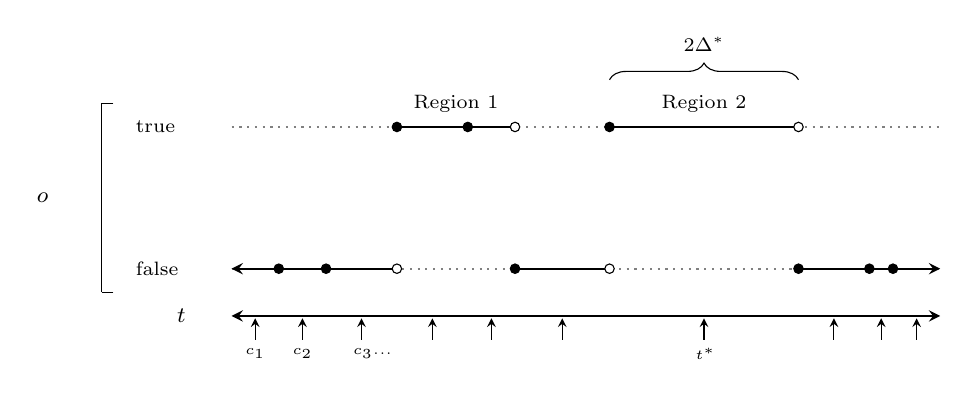
\begin{tikzpicture}[
    axis/.style={thick,<->,>=stealth},
    guide/.style={thick,dotted,gray},
    graphline/.style={thick,black},
    threshmark/.style={thin,->,>=stealth}]

  \def\f{*0.6}

  \draw[axis]
    (1\f,2\f) -- (16\f,2\f);

  \draw[guide]
    (1\f,3\f) -- (16\f,3\f)
    (1\f,6\f) -- (16\f,6\f);

  \draw[graphline,<-,>=stealth]
    (1\f,3\f) -- (4.5\f,3\f);
  \draw[graphline,->,>=stealth]
    (13\f,3\f) -- (16\f,3\f);
  \draw[graphline]
    (4.5\f,6\f) -- (7\f,6\f)
    (7\f,3\f) -- (9\f,3\f)
    (9\f,6\f) -- (13\f,6\f);

  \filldraw[black,draw=black] (2\f,3\f) circle [radius=0.1\f];
  \filldraw[black,draw=black] (3\f,3\f) circle [radius=0.1\f];
  \filldraw[black,draw=black] (4.5\f,6\f) circle [radius=0.1\f];
  \filldraw[black,draw=black] (6\f,6\f) circle [radius=0.1\f];
  \filldraw[black,draw=black] (7\f,3\f) circle [radius=0.1\f];
  \filldraw[black,draw=black] (9\f,6\f) circle [radius=0.1\f];
  \filldraw[black,draw=black] (13\f,3\f) circle [radius=0.1\f];
  \filldraw[black,draw=black] (14.5\f,3\f) circle [radius=0.1\f];
  \filldraw[black,draw=black] (15\f,3\f) circle [radius=0.1\f];
  \filldraw[white,draw=black] (4.5\f,3\f) circle [radius=0.1\f];
  \filldraw[white,draw=black] (7\f,6\f) circle [radius=0.1\f];
  \filldraw[white,draw=black] (9\f,3\f) circle [radius=0.1\f];
  \filldraw[white,draw=black] (13\f,6\f) circle [radius=0.1\f];

%  \draw[threshmark] (1.5\f,3.5\f) -- (1.5\f,3.05\f);
%  \draw[threshmark] (2.5\f,3.5\f) -- (2.5\f,3.05\f);
%  \draw[threshmark] (3.75\f,3.5\f) -- (3.75\f,3.05\f);
%  \draw[threshmark] (5.25\f,6.5\f) -- (5.25\f,6.05\f);
%  \draw[threshmark] (6.5\f,6.5\f) -- (6.5\f,6.05\f);
%  \draw[threshmark] (8\f,3.5\f) -- (8\f,3.05\f);
%  \draw[threshmark] (11\f,6.5\f) -- (11\f,6.05\f);
%  \draw[threshmark] (13.75\f,3.5\f) -- (13.75\f,3.05\f);
%  \draw[threshmark] (14.75\f,3.5\f) -- (14.75\f,3.05\f);
%  \draw[threshmark] (15.5\f,3.5\f) -- (15.5\f,3.05\f);
  
%  \node[align=left] at (1.5\f,3.8\f) {\tiny $o_1$};
%  \node[align=left] at (2.5\f,3.8\f) {\tiny $o_2$};
%  \node[align=left] at (3.75\f,3.8\f) {\tiny $o_3$};
%  \node[align=left,text width=10\f] at (5.25\f,6.8\f) {\tiny $o_4...$};

  \draw[threshmark] (1.5\f,1.5\f) -- (1.5\f,1.95\f);
  \draw[threshmark] (2.5\f,1.5\f) -- (2.5\f,1.95\f);
  \draw[threshmark] (3.75\f,1.5\f) -- (3.75\f,1.95\f);
  \draw[threshmark] (5.25\f,1.5\f) -- (5.25\f,1.95\f);
  \draw[threshmark] (6.5\f,1.5\f) -- (6.5\f,1.95\f);
  \draw[threshmark] (8\f,1.5\f) -- (8\f,1.95\f);
  \draw[threshmark] (11\f,1.5\f) -- (11\f,1.95\f);
  \draw[threshmark] (13.75\f,1.5\f) -- (13.75\f,1.95\f);
  \draw[threshmark] (14.75\f,1.5\f) -- (14.75\f,1.95\f);
  \draw[threshmark] (15.5\f,1.5\f) -- (15.5\f,1.95\f);

  \node[align=left] at (1.5\f,1.2\f) {\tiny $c_1$};
  \node[align=left] at (2.5\f,1.2\f) {\tiny $c_2$};
  \node[align=left,text width=10\f] at (3.75\f,1.2\f) {\tiny $c_3...$};
%  \node[align=left] at (3.75\f,1.2\f) {\tiny $c_3$};
%  \node[align=left,text width=10\f] at (5.25\f,1.2\f) {\tiny $c_4...$};
  \node[align=left,text width=10\f] at (11\f,1.2\f) {\tiny $t^*$};

  \node[align=right,text width=30\f] at (-0.5\f,2\f) {\footnotesize $t$};
  \node[align=left,text width=30\f] at (-0.5\f,3\f) {\scriptsize false};
  \node[align=left,text width=30\f] at (-0.5\f,6\f) {\scriptsize true};

  \draw 
    (-1.5\f,2.5\f) -- (-1.75\f,2.5\f)
    (-1.75\f,2.5\f) -- (-1.75\f,6.5\f)
    (-1.5\f,6.5\f) -- (-1.75\f,6.5\f);

  \node at (-3\f,4.5\f) {\footnotesize $o$};

%  \draw[decorate,decoration={brace,amplitude=10\f},rotate=0] (4.5\f,7\f) -- (7\f,7\f);
  \draw[decorate,decoration={brace,amplitude=10\f},rotate=0] (9\f,7\f) -- (13\f,7\f);

  \node[align=center] at (5.75\f,6.5\f) {\scriptsize Region 1};
  \node[align=center] at (11\f,6.5\f) {\scriptsize Region 2};
  \node[align=center] at (11\f,7.75\f) {\scriptsize $2\Delta^*$};
\end{tikzpicture}
\caption[Operation of the BestInterval algorithm]{Operation of the BestInterval algorithm.  Example values of a binary objective $o(t)$ are shown for a range of input thresholds $t$.  $o$ is a sparse sample of the objective function $f$, evaluated at candidate cutpoints $c$, $o_i = f(w(c_i,d),y)$.  At discrete points defined by observed data values (shown as dots), the objective function $f$ can transition, as an observed data point changes its value relative to $t$, and therefore its assigned class.  Two regions in which $o = \mathrm{true}$ are shown.  BestInterval locates all such regions, selects the one with largest measure on $t$ (margin), and returns its centre and margin as $(t^*, \Delta^*)$.  In this example, the centre and margin of region 2 would be returned.  To ensure that $o$ is sampled at sufficient density, candidate thresholds $c_1, c_2, \dots$ are defined between all consecutive values, and beyond the extrema, of $x$; these are indicated by small arrows.}
\label{fig:mess-bestinterval}
\end{figure}


\section{Results}
In the following, the performance of Messina2 is characterised through simulation, and its behaviour compared to alternative techniques.  \gls{PDAC} outcome cohorts are used to demonstrate that prognostic biomarkers identified by Messina2 are more likely to validate in external cohorts than those identified by the \texttt{maxstat} method.  Finally, Messina2 is applied to \gls{PDAC} prognostic data from the \gls{APGI}, to identify biomarkers that may form better preoperative measures of prognosis than those used in \Cref{chap:nomogram}.

\subsection{Large-margin classifiers are more robust}
We consider a simple technology translation scenario in which a diagnostic classifier developed on one platform is moved to another.  The classifier is based on the abundance of biomarker $x$, which is used to predict disease state $y \in \{0, 1\}$, by comparing $x$ against a threshold $t$, $\hat{y_i} = [x_i \geq t]$.  Suppose that $t$ was originally derived from many measurements of $x$ made on one measurement platform, as $x_i = D y_i + \epsilon_i$, $\epsilon_i \sim \mathcal{N}(0, 1)$ is the measurement error of the platform.  No generality is lost by forcing the error to be standard normal, as this situation can be achieved simply by scaling $D$.  We use the link between margin and the distribution of $x, y$ for objective $f_M$ (\fref{fig:mess-class-cdf-link}) to derive an expression for the margin of this original classifier.  Given a minimum desired sensitivity and specificity of $0.9$ each, the Messina2 classifier trained on sufficient samples of $x, y$ will have $t = \frac{1}{2}D$ and $\Delta = \frac{1}{2}(\Phi^{-1}(1-0.9)+D-\Phi^{-1}(0.9)) \approx \frac{1}{2}D - 1.28$.  Messina2 will not return a classifier with a non-positive margin, so $\Delta > 0 \Rightarrow D > 2.56$ for this example.

The classifier described above is now to be applied on a new measurement platform, and we are interested in determining how its performance will be affected by this change.  It is reasonable to expect that the new platform will be calibrated to approximately match the original, so that no significant translation or scaling of the values of $x$ will occur.  However, the post-calibration error of the new platform may be very different from that of the old, and this disparity can't be easily corrected.  Let the measurements of $x$ on the new platform be $x'_i = D y_i + \epsilon'_i$, with $\epsilon'_i \sim \mathcal{N}(0, \sigma'^2)$, and the predictions on the new platform be $\hat{y'_i} = [x'_i \geq t]$.  Our intent is to characterise how the error rate of $\hat{y'}$ changes as a function of $\Delta$ and $\sigma'$.  False positives will occur when $\epsilon'_i \geq t$, and false negatives when $D + \epsilon'_i < t$; these two error types together will occur at a rate of
\begin{align*}
R_E &= f_0\left(1-\Phi\left(\frac{t}{\sigma'}\right)\right) + f_1\left(\Phi\left(\frac{t-D}{\sigma'}\right)\right) \\
    &= f_0\left(1-\Phi\left(\frac{D}{2\sigma'}\right)\right) + f_1\left(\Phi\left(-\frac{D}{2\sigma'}\right)\right) \\
    &= \Phi\left(-\frac{D}{2\sigma'}\right) \\
    &= \Phi\left(-\frac{\Delta}{\sigma'} - \frac{1.28}{\sigma'}\right)
\end{align*}
where $f_0$ and $f_1$ are the relative proportions of class 0 and 1 in the test population; these disappear from the expression following simplification.

In this simulation, the total error rate therefore increases with increasing measurement error $\sigma'$, and decreases with increasing margin $\Delta$: as intuitively expected, classifiers with higher margin are more robust to measurement error.  This is shown in \fref{fig:mess-margin-good}, in which increasing margin can be seen to offset the increase in error rate caused by a high $\sigma'$.

\begin{figure}[!htbp]
\centering
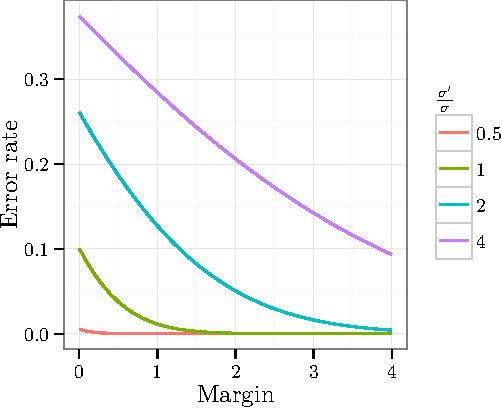
\includegraphics[width=.7\linewidth]{analysis/messina/figure/05-E1-E1A3-1}
\caption[TODO]{TODO}\label{fig:mess-margin-good}
\end{figure}

\subsection{Messina2 provides accurate control over classifier margin}
High-margin classifiers are desirable due to their robustness, but is Messina2 effective in building classifiers with the desired margin, and how does this compare to other techniques?  To address this, Messina2 and representative other techniques were applied to simulated diagnostic and prognostic data.  Methods were compared for sensitivity -- the rate at which they detected simulated biomarkers with desired characteristics -- and specificity -- the rate at which they rejected simulated biomarkers that lacked desired characteristics.

\paragraph{Classification ($f_M$)}
Messina2 with an $f_M$ objective was compared to the t-test.  Simulated $x_i$ were drawn from a normal distribution, as $x_i \sim \mathcal{N}(D y_i, 1)$, with $D \in [0, 5]$ and $y \in \{0, 1\}$.  Classes were balanced, so that near-equal numbers of $y = 0$ and $y = 1$ samples were present in all runs.  The total number of samples in a run, $n$, was either 25, 50, or 100.  For each combination of $D$ and $n$, \fcardinal{1000} random cohorts were generated and supplied to Messina2 and the t-test, and detection rates recorded.  Messina2's $f_M$ parameters were $l_n \geq 0.8$, $l_c \geq 0.8$, and $\Delta \geq 1$, and the t-test was used with a size ($\alpha$) of $0.05$.

Across all sample sizes, Messina2 consistently only selected a biomarker when its true margin was near the target value of 1 (\fref{fig:mess-vs-t}).  Conversely, the t-test was far less selective, identifying even biomarkers with a zero margin as being differentially-expressed.  This sensitivity to small differences, particularly in large samples, is a concrete example of the effect illustrated in \fref{fig:messina-example-stats-class}: a statistically significant result does not necessarily indicate that a good classifier can be made.  The result of this simulation suggests that if the t-test were used to identify single-gene diagnostic biomarkers, a very high false positive rate could be expected, and many of the reported biomarkers would lead to small-margin classifiers that would be unlikely to be robust.  This effect only becomes more pronounced as the sample size increases.

\begin{figure}[!htbp]
\centering
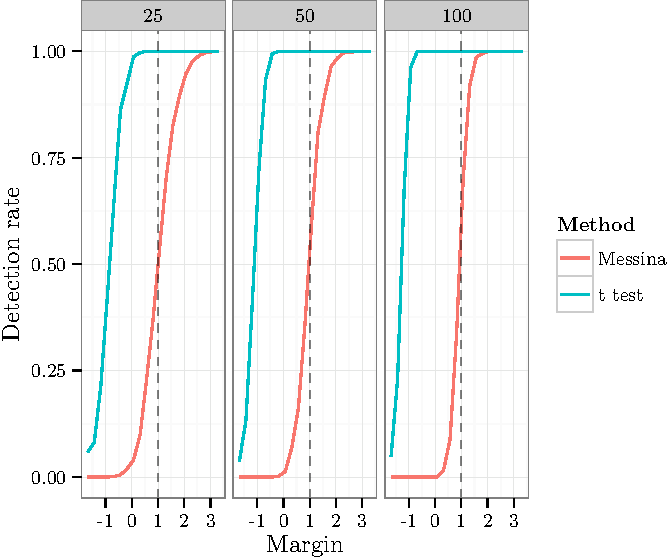
\includegraphics[width=\linewidth]{analysis/messina/figure/06-E2A-E2A-plots-1}
\caption[TODO]{TODO}\label{fig:mess-vs-t}
\end{figure}

\paragraph{Prognosis ($f_H$)}
Messina2 using the $f_H$ objective function was compared to the \texttt{maxstat} corrected optimal cut procedure, and the simple median-cut log-rank test.  Simulated data were generated in a similar fashion to the $f_M$ test above, as follows.  Simulated $x_i$ were drawn as $x_i \sim \mathcal{N}(D s_i, 1)$, $D \in [0, 5]$, and $c_i \in \{0, 1\}$ the class membership indicator.  The fraction of class 1 in the sample was either $0.2$ or $0.5$, with simulated data sets containing either 25, 50, or 100 samples.  Event times were sampled from an exponential distribution with rate $4 c_i$, and censoring times from an exponential distribution, with rate calculated to give an expected censoring rate of $0.2$~\footnote{A number of values of the censoring fraction were tested, which for reasonable levels was observed to have only minor effects on results (data not shown)}.  500 simulations were performed for each unique combination of parameters.  Messina2's $f_H$ arguments were $l_h \geq 2$ and $\Delta \geq 1$, and \texttt{maxstat} was used with test \texttt{"LogRank"} and correction method \texttt{"HL"}.  For \texttt{maxstat} and the median-cut, a biomarker was considered detected if its corrected P-value was less than $0.05$.

The detection results on these simulated data are shown in \fref{fig:mess-vs-maxstat}.  Messina2 was not as reliable at controlling classifier margin in these prognostic data as it was in the classification case (\fref{fig:mess-vs-t}); this discrepancy may be due to the greater uncertainty inherent in censored data.  Despite this, Messina2 remained competitive with the other cut optimization procedure \texttt{maxstat}, particularly in small samples.  Messina2 was also substantially faster than \texttt{maxstat}, taking $0.41$ seconds per biomarker for 100 samples, versus $4.80$ seconds for \texttt{maxstat}.  As expected, the median cut procedure was very sensitive when the survival subgroups were balanced, but performed very poorly otherwise.

\begin{figure}[!htbp]
\centering
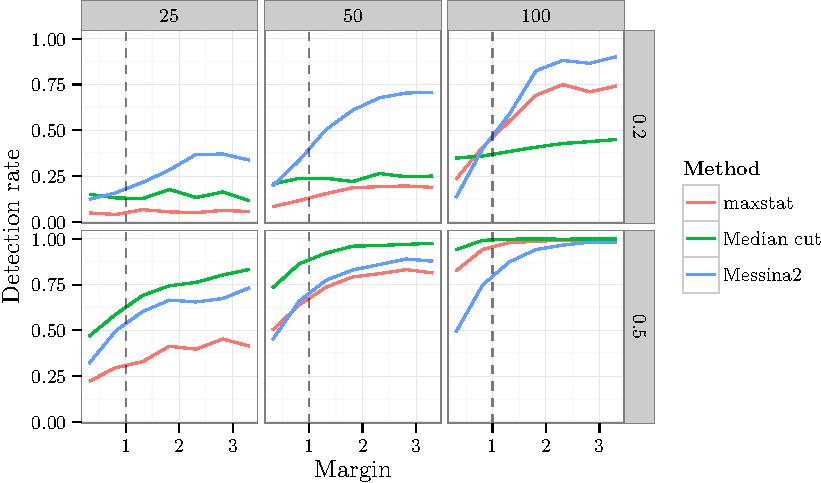
\includegraphics[width=\linewidth]{analysis/messina/figure/06-E2B-E2B-plots-1}
\caption[TODO]{TODO}\label{fig:mess-vs-maxstat}
\end{figure}

\subsection{Messina2 is more effective than maxstat at finding validating biomarkers}
The above development of Messina2 contains some heuristic arguments for classifiers with large margins, but 

that classifiers with large margins are more likely to be accurate in 

for a high classifier margin being desirable

various heuristic arguments have 

\subsection{Application of Messina2 to identify biomarkers for \acrshort{PDAC} prognosis}

\section{Discussion}

\section{Methods}




\begin{figure}[!htbp]
\centering
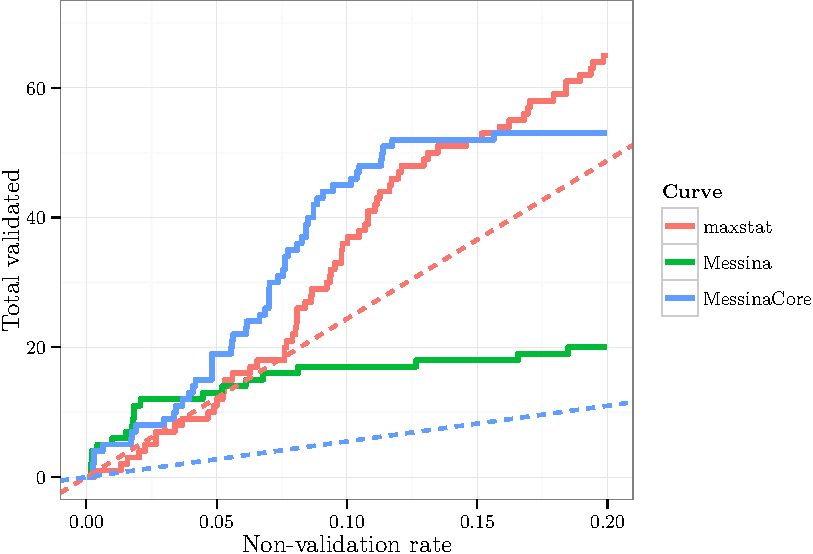
\includegraphics[width=.7\linewidth]{analysis/messina/figure/07-E3-E3-val-detcurves-1}
\caption[]{}\label{fig:mess-val-detabs}
\end{figure}

\begin{figure}[!htbp]
\centering
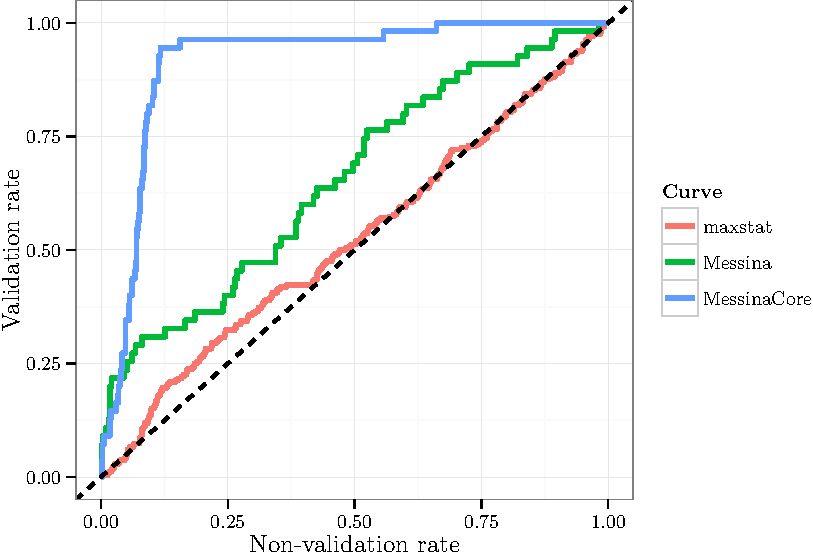
\includegraphics[width=.7\linewidth]{analysis/messina/figure/07-E3-E3-val-detcurves-2}
\caption[]{}\label{fig:mess-val-detrel}
\end{figure}


TODO: ADVANTAGE OVER ROC.  See above para.  So basically, someone might argue -- why not just do a ROC with a cost-sensitive threshold?  That way it can be done with any classifier that gives a continuous output.  Problem is that the ROC doesn't include margin information.  So it's not just about hitting the right balance of sens & spec, but doing so ROBUSTLY.  How sure can we be that our target sens & spec will be achieved on a test set?  What about a completely different cohort?  Using a different technology?  Best option is to MAXIMIZE MARGIN.  I need to put this thinking somewhere.  TODO: DISCUSSION

\end{document}
